
%%%%%%%%%%%%%%%%%%%%%% Chapter 2.1
\chapter{Introductory Examples}


\section{Direct Current and Circuit Laws}

Current is the flow of chare. We will look at it as conventional current (positive flow). Voltage and current are constant for \Emph{direct current} (DC). Two various types of two-terminal circuits elements may be classified according to their terminal voltage-current $v(i)$ relationships: \begin{itemize}
    \item $v(i) = $ constant
    \item $v = v(t), i = i(t)$ - ideal voltage source (independent voltage source)
\end{itemize}

\begin{defn}
    The waveform $v(t)$ represents the voltage produced by the source. ``Ideal source" means the voltage is maintained regardless of the drawn current.
\end{defn}

\begin{defn}
    An \Emph{ideal battery} has its voltage drop between the terminals being $V_0$.
\end{defn}

\begin{figure}[H]
    \centering
    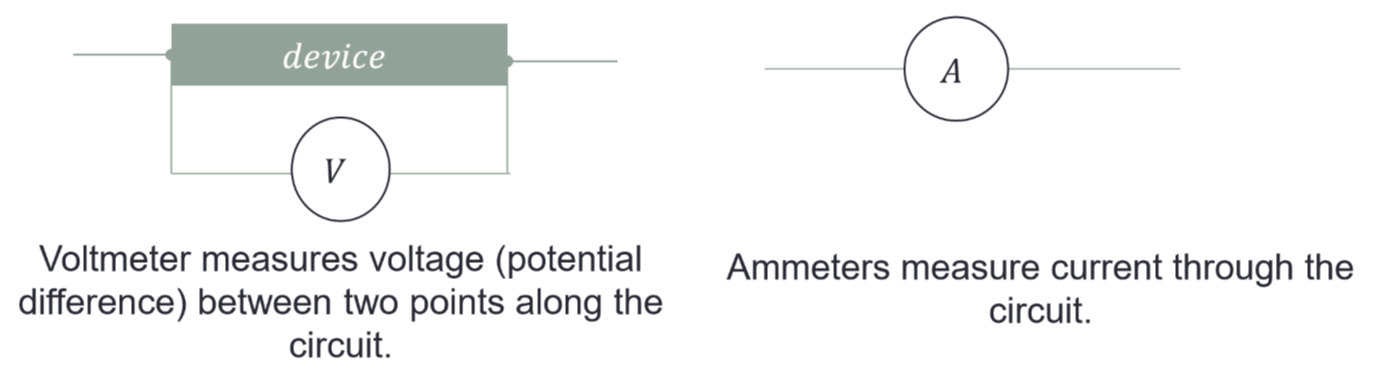
\includegraphics[scale = 0.6]{Images/TH1.PNG}
\end{figure}

\begin{defn}[Ohm's Law]
    \Emph{Ohm's Law} states that for a resistor connected between terminals $A$ and $B$, the voltage drop from $A$ to $B$ is equal to the resistance multiplied by the current flowing from $A$ to $B$ through the resistor. \begin{equation*}
        I = \frac{V}{R}\implies V = IR
    \end{equation*}
    and \begin{equation*}
        v(t) = Ri(t)\implies i(t) = \frac{1}{R}v(t)
    \end{equation*}
    for \Emph{ohmic materials} (such as wires)
\end{defn}

\subsection{Resistance}

Resistance depends on the geometry and the material of the conductor. For a specific temperature, $R \propto \frac{L}{A}$, specifically \begin{equation*}
    R = \rho\frac{L}{A}
\end{equation*}
where $\rho$ is the \Emph{resistivity} ($\Omega m$).

\begin{table}[H]
    \centering
    \caption{Material Resistivity}
    \begin{tabular}{|cc|}
        \hline 
        Material & Resistivity $\Omega m$ \\ \hline
        Silver & $1.59\times 10^{-8}$ \\ \hline
        Copper & $ 1.68\times 10^{-8}$ \\ \hline 
        Aluminum & $2.65\times 10^{-8}$ \\ \hline
        Tungsten & $5.6\times 10^{-8}$ \\ \hline
        Graphite & $(3$-$60)\times 10^{-5}$ \\\hline
        Silicon & $0.1-60$ \\ \hline
        Hard Rubber & $(1$-$100)\times 10^{13}$ \\ \hline
    \end{tabular}
\end{table}

\begin{defn}
    The power absorbed by a resistor can be calculated according to \begin{equation*}
        P(t) = v(t)i(t) = i^2(t)R = \frac{v^2(t)}{R}
    \end{equation*}
\end{defn}
For DC current this reduces to $P = IV = I^2R = \frac{V^2}{R}$.

\subsection{Circuit Laws}

\begin{thm}[Kirchhoff's Current Law]
    The algebraic sum of all the currents entering and leaving a node is equal to zero. \begin{equation*}
        \sum_{i=1}^nI_i = 0
    \end{equation*}
    \begin{figure}[H]
        \centering
        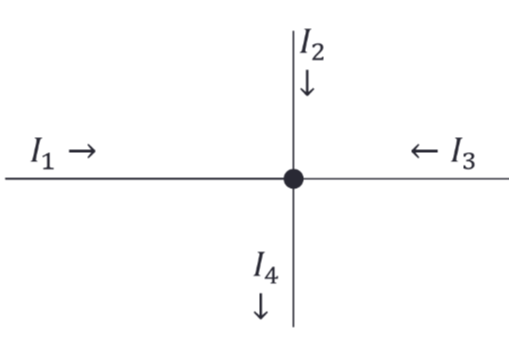
\includegraphics[scale = 0.8]{Images/TH2.PNG}
    \end{figure}
    This is really \Emph{conservation of charge}.
\end{thm}

\begin{thm}[Kirchhoff's Voltage Law]
    The algebraic sum of all the voltage drops around any closed path is zero at every distance and time: \begin{equation*}
        \sum_{i=1}^nV_i = 0
    \end{equation*}
    This is a form of \Emph{energy conservation}.
\end{thm}

For a circuit and any pair of nodes $j$ and $k$, the voltage drop $v_{jk}$ from node $j$ to node $k$ is $$v_{jk} = v_j - v_k$$


\begin{thm}[Resistors in Series]
    If we have a line of $n$ resistors in series (i.e. the same current passes through all of them), then the equivalent resistance of the collection is their sum: $$R_{eq}^{series} = \sum_{i=1}^nR_i$$
    \begin{figure}[H]
        \centering
        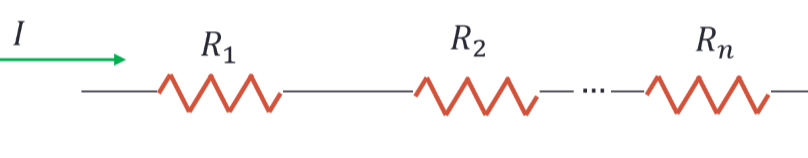
\includegraphics[scale = 0.8]{Images/TH3.PNG}
    \end{figure}
\end{thm}

Now, consider a circuit that has $n$ resistors in series connected to a battery, $V_{in}$, with current $I$. Then the equivalent resistance across the series of resistors is $R_{eq} = V_{in}/I$, so the voltage drop across any individual resistor $V_i$ is $$V_i = R_iI = R_i \frac{V_{in}}{\sum_{j=1}^nR_j}$$

\begin{defn}
    $n$ resistors are said to be in parallel if the same voltage drop happens across them:
    \begin{figure}[H]
        \centering
        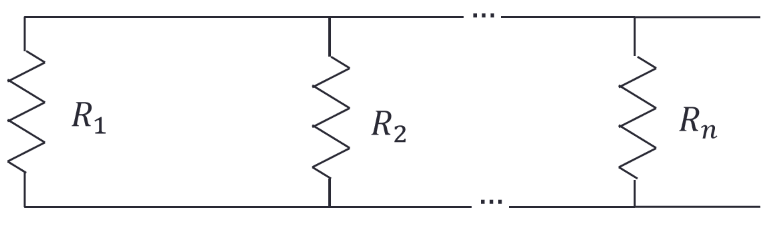
\includegraphics[scale = 0.8]{Images/TH4.PNG}
    \end{figure}
    In this case different currents go through each resistor, say current $I_i$ goes through resistor $R_i$, and we have $$I_T = \frac{V_{in}}{R_{eq}} = \sum_{i=1}^nI_i = \sum_{i=1}^n\frac{\Delta V_i}{R_i}$$ where by Kirchhoff's voltage law $V = \Delta V_i$ for each $I$, so $$\frac{1}{R_{eq}} = \sum_{i=1}^n\frac{1}{R_i}$$
\end{defn}

\subsection{Voltmeters and Ammeters}

\begin{defn}
    A voltmeter measures voltage (potential difference) between two points along the circuit. We connect them in \Emph{parallel} to the device. To connect them we create a node, which means some current will always go through the resistor. The goal is to send as little current as possible through the voltmeter, therefore voltmeters have \Emph{very high internal resistances}.
\end{defn}

\begin{defn}
    Ammeters measure current through the circuit. We connect them in \Emph{series} with other elements. In order not to affect the circuit, we want them to have the smallest internal resistance possible.
\end{defn}

\subsection{Th\'{e}venin Theorems}

\begin{thm}
    Given an arbitrary two-terminal linear network $N$ consisting of resistances and independent sources, then, for almost all such $N$, there exists an equivalent two-terminal network consisting of a resistance $R_{th}$ in series with an independent voltage source $V_{oc}(t)$.
\end{thm}

The voltage $V_{oc}(t)$ (open-circuit voltage) is what appears across the two terminals of $N$ when no other network is attached. Resistance $R_{th}$ (Th\'{e}venin Equivalent Resistance) is the equivalent resistance of $N$ when all independent sources are deactivated.

The procedure for calculations is as follows:

\begin{enumerate}
    \item Remove the load resistor $R_L$ or component concerned. (Create an opening between two terminals)
    \item Remove the active sources: Remove voltage sources by shortening them, and remove current sources by opening them
    \item Find $R_{th}$ using rules for regular equivalent resistances.
    \item Find $V_{oc}$ by the usual circuit analysis methods.
    \item Find the current flowing through the load resistor $R_L$.
\end{enumerate}


\section{RLC Circuits}

\subsection{Phasors}

First recall we can consider an oscillation $s(t) = A\cos(\omega t+\phi_0)$ as the real part of a complex function $$\tilde{s}(t) = Ae^{i(\omega t+\phi_0)}$$ Similarly, $y(t) = A\sin(\omega t+\phi_0)$ can be seen as the imaginary part of the same function. $\tilde{s}(t)$ is our \Emph{phasor}. Note that waves add as phasors, which add vectorally (superposition principle). In general, any oscillation can be broken into a sum of simple harmonic oscillations (i.e. Fourier series). 


\subsection{Capacitors}

Now, the capacitor usually consists of a pair of parallel plates (possibly with a dielectric between them) storing opposite charges on either side, and hence containing a potential difference between the plates.

\begin{defn}
    \Emph{Capacitance} is the ratio of the magnitude of the charge on one of the plates of the capacitor to the absolute value of the potential difference between them is defined as \begin{equation*}
        C = \frac{q}{|\Delta V|},\;\;1\;F = \frac{1\;C}{1\;V}
    \end{equation*}
\end{defn}
For a parallel-plate capacitor of area $A$ and plate separation $d$ we can compute the capacitance by applying Gauss's Law $\oint\vec{E}\cdot d\vec{A} = \frac{q_{in}}{\varepsilon_0}$, by $$\oint\vec{E}\cdot d\vec{A} = EA = \frac{q}{\varepsilon_0} = \frac{\sigma A}{\varepsilon_0}$$ so $E = \frac{\sigma}{\varepsilon_0}$, so $\Delta V = Ed = \frac{\sigma d}{\varepsilon_0} = \frac{qd}{A\varepsilon_0}$, and $C = \frac{A\varepsilon_0}{d}$.

In order to determine the electric potential energy stored in a capacitor, we look at energy required to transfer charge from one conductor to another. Consider moving an infinitesimal amount of charge $dq'$, so the potential difference is essentially constant during the transfer of one increment $dU^E = -dW = Vdq' = \frac{q'}{C}dq'$, so $U^E = \frac{1}{2}\frac{q^2}{C} = \frac{1}{2}C\Delta V^2 = \frac{1}{2}q\Delta V$.

\subsection{Inductor}

A consequence of Faraday's Law, $\oint \vec{E}\cdot d\vec{l} = -\frac{d\Phi_B}{dt}$, where $\Phi_B$ is the magnetic flux, is that when a current through a conducting loop changes it induces an emf (potential difference, $\varepsilon_{ind}$) in the loop itself. \Emph{Inductance} $L$ of the loop (or solenoid) is defined as a proportionality constant between the emf andthe rate of change of current: $$\varepsilon = -L\frac{dI}{dt},\;\;\;1\;H = \frac{1\;Vs}{1\;A}$$
A device that has an appreciable inductance is called an \Emph{inductor}. It describes the change of magnetic flux associated with a change of current in a particular loop/solenoid.

Work must be done on an inductor to establish the current through it because the change in current causes an induced emf that opposes this change. Consider $dW$, work done \emph{on} the inductor when an amount of charge $dq$ is being moved through it, so $dW = -\varepsilon dq$, $\frac{dW}{dt} = -\varepsilon I = LI\frac{dI}{dt}$, and so $W = \int dW = \frac{1}{2}LI^2$ and $U^B = \frac{1}{2}LI^2$.

\subsection{AC Current}

For a conductor, at any instance $C = \frac{q}{v_c(t)}$ so $q = Cv_c(t) = CV_c\sin(\omega t)$. Current is $$i(t) = CV_c\omega \cos(\omega t) = CV_c\omega\sin\left(\omega t + \frac{\phi}{2}\right) = I_c\sin\left(\omega t+\frac{\phi}{2}\right)$$ As $I_C = CV_C\omega$, $V_C = \frac{I_C}{C\omega}$, so $Z_C = \frac{1}{\omega C}$.

First, $v_L(t) = L\frac{di}{dt} = V_L\sin(\omega t)$, so $$i(t) = -\frac{V_L}{\omega L}\cos(\omega t) = \frac{V_L}{\omega L}\sin\left(\omega t -\frac{\pi}{2}\right)$$ Then $$I_L = \frac{V_L}{\omega L}\implies Z_L = \omega L$$

\subsection{Series RLC Circuit}

First, for a circuit consisting of an inductor, resistor, capacitor, and an AC voltage source, we have the relation $\varepsilon = v_R(t) + v_L(t) + v_C(t)$. Current is the same for all three elements, so $$V_0\sin(\omega t) = \frac{1}{C}\int idt + L\frac{di}{dt}+iR$$ and differentiating $$V_0\omega \cos(\omega t) = \frac{i}{C} + L\frac{d^2i}{dt^2} + R\frac{di}{dt}$$ The solution to these DEs is $$i(t) = \frac{V_0\sin(\omega t-\phi)}{\sqrt{R^2 + \left(\omega L - \frac{1}{\omega C}\right)^2}}$$ where $$\phi = \tan^{-1}\left[\frac{\omega L - \frac{1}{\omega C}}{R}\right]$$




%%%%%%%%%%%%%%%%%%%%%% Chapter 2.2
\chapter{AC Sources, Waveforms}

Recall that ``AC" stands for \Emph{alternating current} - current whose value oscillates sinusoidally about a mean value of zero through time. Recall also from Fourier transform theory that any well-behaved signal of any shape can be synthesized as a linear combination of pure AC signals of appropriately chosen frequencies, amplitudes, and phases.

First, in a circuit diagram we notate an AC voltage source by:

\begin{figure}[H]
    \centering
    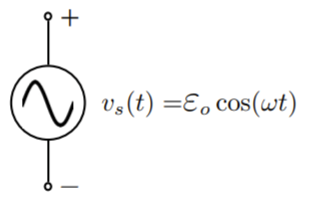
\includegraphics[scale = 0.8]{Images/ACSymbol.PNG}
    \caption{Circuit symbol for an ideal AC voltage source. $\pm$ signs show the polarity of the output voltage at $t = 0$.}
    \label{fig:ACSymb}
\end{figure}

The defining property of an ideal AC voltage source is that it produces a sinusoidally varying voltage signal of constant amplitude and frequency across its terminals, no matter what device is connected across them $$v_s(t) = v_+ - v_- = \varepsilon_0\cos(\omega t)$$
where $\varepsilon_0$ and $\omega$ are positive real constants. $\varepsilon_0$ is the constant \Emph{voltage amplitude} of the source, measured in volts $(V)$ SI units. $\omega$ is the \Emph{angular frequency} of the source, measured in radians per second. The waveform executes one complete cycle in a time interval equal to the period $T$: $$T = \frac{1}{f} = \frac{2\pi }{\omega}$$ This is illustrated in the Figure:

\begin{figure}[H]
    \centering
    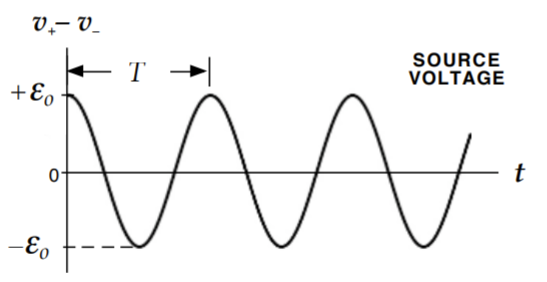
\includegraphics[scale = 0.8]{Images/ACVoltageSource.PNG}
    \caption{Output voltage signal of the ideal AC voltage source of Figure \ref{fig:ACSymb}.}
    \label{fig:ACSource}
\end{figure}

Often we will ground the lower terminal of an ideal voltage source, so that all potentials in the circuit are measured relative to that ground. 

\begin{defn}
    The \Emph{root-mean-square voltage}, or $V_{rms}$, of an AC voltage source is the square root of the time-averaged square of the voltage signal. For the AC voltage source this is just $$V_{rms} = \frac{1}{\sqrt{2}}\varepsilon_0$$
\end{defn}

Sometimes the amplitude will be given in terms of the rms voltage. A third way of specifying the voltage amplitude is the \Emph{peak-to-peak voltage swing}, or maximum voltage minus minimum voltage for one cycle of the voltage waveform. For an AC waveform this is simply twice the amplitude.

\section{Loaded Ideal AC Voltage Generator}

Consider the AC circuit in which an ideal AC voltage source of the type described previously is connected across a circuit element, referred to as the \Emph{load}. The load is a ``black box" with two terminals. If the load contains only some combination of inductance, resistance, and capacitance, then it is said to be a \Emph{passive linear load}.

\begin{prop}
    When considering an AC circuit with a passive linear load as the only component, the laws of physics dictate that the current $i(t)$ in the circuit must be a constant-amplitude sinusoidal function of time with the same angular frequency as the ideal voltage source: $$i(t) = I_0\cos(\omega t+\phi)$$
    $I_0$ is the \Emph{current amplitude}, measured in amperes $(A)$, and $\phi$ is the \Emph{phase angle}.
\end{prop}

When the load is \Emph{pure resistance} $R$, the law of the resistor dictates that $v_s = iR$ (Ohm's Law). Thus, in the resistive case, $\phi = 0$, the current has amplitude $I_0 = \frac{\varepsilon_0}{R}$, and the current is exactly in phase with the source voltage $v_s(t)$. THe presence of capacitors and/or inductors is what gives us a phase shift.

\section{Three Fundamental Circuits}

An important problem in AC circuit theory is finding the current in the circuit when the load network is specified. We shall first investigate the simple case where the load consists of a single fundamental circuit element: a resistor, a capacitor, or an inductor. In the case of a resistor, we have the following law:

\begin{thm}[Law of the Resistor]
    The voltage across a resistor is given by $$v_R(t) = i(t)R$$ Putting $v_R = v_s(T) = \varepsilon_0\cos(\omega t)$, we obtain $$i(t) = \frac{\varepsilon_0}{R}\cos(\omega t)$$ Thus, we have current amplitude $I_0 = \frac{\varepsilon_0}{R}$ and current phase $\phi = 0$.
\end{thm}

For a capacitor we have the following law:

\begin{thm}[Law of the Capacitor]
    The voltage across a capacitor with capacitance $C$ and storing charge $q(t)$ is $$v_C(t) = \frac{q(t)}{C}$$ or $$i(t) = \frac{dq}{dt} = C\frac{dv_C}{dt}$$ With $v_C = v_s(t) = \varepsilon_0\cos(\omega t)$, $i(t)$ is $$i(t) = -\omega C\varepsilon_0\sin(\omega t) = \omega C\varepsilon_0\cos(\omega t+\pi/2)$$ The current amplitude is $I_0 = \omega C\varepsilon_0$, and the current phase is $\phi = \pi/2$.
\end{thm}

Finally, the law for inductors is as follows:

\begin{thm}[Law of the Inductor]
    The voltage across an inductor with inductance $L$ is given by $$v_L(t) = L\frac{di(t)}{dt}$$ or $$i(t) = \frac{1}{L}\int_0^tv_L(t')dt'$$ Putting $v_L = v_s(t) = \varepsilon_0\cos(\omega t)$ and solving for $i(t)$ gives $$i(t) = \frac{\varepsilon_0}{\omega L}\sin(\omega t) = \frac{\varepsilon_0}{\omega L}\cos(\omega t - \pi/2)$$ The current amplitude is $I_0 = \frac{\varepsilon_0}{\omega L}$ and the current phase is $\phi = -\pi/2$.
\end{thm}

We can summarise these results as follows: \begin{itemize}
    \item When an AC voltage signal of amplitude $V_0$ and angular frequency $\omega$ appears across any linear circuit element, the current in the element is guaranteed to be an AC current signal of the same angular frequency $\omega$ as the voltage signal.
    \item When the device is a \Emph{resistor} of resistance $R$, the current is exactly in phase with the voltage across the resistor $(\phi = 0)$, and the current amplitude is given by $I_0 = V_0/R$.
    \item When the device is a \Emph{capacitor} of capacitance $C$, the current is $\pi/2$ radians ahead of the voltage across the capacitor $(\phi = \pi/2)$; the current amplitude is frequency dependent and given by $I_0 = \omega CV_0$
    \item When the device is an \Emph{inductor} of capacitance $C$, the current is $\pi/2$ radians behind the voltage across the inductor $(\phi = -\pi/2)$; the current amplitude is frequency dependent and given by $I_0 = V_0/(\omega L)$
\end{itemize}

Note that in the case of a conductor, \Emph{the source voltage directly determines the charge on the upper plate of the capacitor}, not the current, as was the case with the resistive load. The current is then the resulting time derivative of the capacitor charge $q$. Indeed, the current is the scaled derivative of the source voltage. 


%%%%%%%%%%%%%%%%%%%%%% Chapter 2.3
\chapter{Phasor Analysis}

A \Emph{phasor} is simply a complex number, a constant independent of time, that contains information on both the amplitude and phase of the AC signal. 

\section{Phasors and Complex Sinusoids}

Recall that we can use Euler's relation to express a complex exponential as $$e^{j\theta} = \cos\theta + j\sin\theta$$ where $j = \sqrt{-1}$, and that the modulus of $e^{j\theta}$ is $1$. If we set $j\theta = j\omega t$ we will have made what is called a time-dependent \Emph{complex sinusoid of unit amplitude}, $e^{j\omega t}$.

Recall that for a single loop circuit, one with a linear load, we have the current $$i(t) = I_0\cos(\omega t+\phi)$$ 

\begin{defn}
    We define the time-independent \Emph{complex amplitude} or \Emph{phasor} associated with $i(t)$ as $$\hat{I} = I_0e^{j\phi}$$
    Combining the phasor $\hat{I}$ with the complex sinusoid $e^{j\omega t}$ we can express the current as $$i(t) = \text{Re}\left(\hat{I}e^{j\omega t}\right) = I_0\cos(\omega t+\phi)$$
\end{defn}

Using our phasor $\hat{I}$, we can recover the amplitude and phase of the physical current as follows: $$I_0 = |\hat{I}| = \sqrt{(\text{Re}\hat{I})^2+(\text{Im}\hat{I})^2};\;\;\;\phi = \tan^{-1}\left[\frac{\text{Im}\hat{I}}{\text{Re}\hat{I}}\right]$$

\section{Kirchhoff's Rules}

\begin{thm}[Kirchhoff's Point Rule]
    For any junction in a circuit with $n$ currents going into it, $i_1(t),...,i_n(t)$, where $i_j(t) < 0$ if it is conventional current going out of the junction, and $i_j(t) > 0$ if it is conventional current going into the junction, then $$\sum_{j=1}^ni_j(t) = 0$$ This is a statement of conservation of charge.
\end{thm}

If this junction is part of a circuit network driven by a single AC voltage source of angular frequency $\omega$, each of the currents will itself be a sinusoidal function of time with the same angular freuency $\omega$ as the source. Using complex phasor amplitudes, $\hat{I}_k = I_ke^{j\phi_k}$, we have that $$\text{Re}\left[\sum_{k=1}^n\hat{I}_ke^{j\omega t}\right] = 0$$ First, note that $\sum_{k=1}^n\hat{I}_k = \sum_{k=1}^nI_ke^{j\phi_k} = I_Se^{j\phi_S}$ for some $I_S$ and $\phi_S$ since all complex numbers can be expressed in polar form. Then $\text{Re}\left[I_Se^{j\phi_S}e^{j\omega t}\right]  = 0$. Since this holds for all $t$, we must have that $I_S = 0$ (setting $t = \frac{-\phi_S}{\omega}$), and it follows that $I_Se^{j\phi_S}e^{j\omega t} = 0$. Thus we have the complex equation $$\sum_{k=1}^n\hat{I}_ke^{j\omega t} = \sum_{k=1}^nI_ke^{j\phi_k}e^{j\omega t} = 0$$ Since $e^{j\omega t} \neq 0$, this is equivalent to the following:

\begin{thm}[Kirchhoff's point rule (phasors)]
    Kirchhoff's point rule is equivalent to $$\sum_{k=1}^n\hat{I}_k = \sum_{k=1}^nI_ke^{j\phi_k} = 0$$ where $\hat{I}_k$ is the phasor of the $k$th current going into the junction.
\end{thm}

\noindent Next we have Kirchhoff's loop rule:

\begin{thm}[Kirchhoff's Loop Rule]
    If one encounters $n$ voltage drops/gains, $v_k(t)$, when going around a closed loop with zero resistance wires, Kirchhoff's loop rule state $$\sum_{k=1}^nv_k(t) = 0$$ This is a statement of the law of conservation of energy.
\end{thm}

If the voltage drops are AC signals of phasor amplitudes $\hat{V}_k = V_ke^{j\phi_k}$, the loop rule can be transformed as with the junction rule:

\begin{thm}[Kirchhoff's Loop Rule (phasors)]
    Kirchhoff's loop rule is equivalent to $$\sum_{k=1}^n\hat{V}_k = \sum_{k=1}^nV_ke^{j\phi_k} = 0$$ where $\hat{V}_k$ is the phasor of the $k$th voltage drop/gain, if all voltage drops/gains are AC signals with the same angular frequency $\omega$.
\end{thm}

\section{Phasor Summary}

We summarize the properties of phasors as follows: 

\begin{itemize}
    \item A \Emph{phasor} is a complex constant (no time dependence) associated with a voltage or current waveform in an AC circuit.
    \item Any complex number $z = x+jy$ can be written in polar form $z = |z|e^{j\phi}$ with $\phi$ its phase constant or argument, and $|z|$ its modulus or magnitude.
    \item For an AC current signal $i(t) = I_{max}\cos(\omega t+\phi)$, the associated phasor is $\hat{I} = I_{max}e^{j\phi}$. If we have the phasor $\hat{I}$ we can recover the amplitude and phase of $i(t)$ as $I_{max} = |\hat{I}|$ and $\phi = \text{arg}\hat{I}$.

        Similarly, for any AC voltage signal $v(t) = V_{max}\cos(\omega t+\theta)$, the associated phasor is $\hat{V} = V_{max}e^{j\theta}$. If we have the phase $\hat{V}$ we can recover the amplitude and phase of $v(t)$ as $V_{max} = |\hat{V}|$ and $\theta = \text{arg}\hat{V}$.
    \item When phasors add, their real and imaginary parts add to produce the phasor sum.
\end{itemize}

Recall that complex numbers behave exactly like two-dimensional real vectors under addition. We can use this fact to draw vector addition diagrams, called \Emph{phasor addition diagrams} in our context.


\section{Complex Impedance}

Consider a circuit consisting of an ideal AC voltage source of frequency $f$ connected across a load containing nothing but capacitors, resistors, and inductors, connected to each other in some arbitrary fashion. Such a load is called a \Emph{passive linear load}, since it contains no sources of emf. Recall that in this case $v(t) = \varepsilon_0 \cos\omega t$ and $i(t) = I_{max}\cos(\omega t+\phi)$. The phasors, $\hat{V}$ and $\hat{I}$, representing the load are $\hat{V} = \varepsilon_0$ and $\hat{I} = I_{max}e^{j\phi}$. 

\begin{defn}
    The \Emph{complex impedance} $Z$ of a load is the ratio of its voltage phasor to its current phasor: $$Z = \frac{\hat{V}}{\hat{I}}$$ The unit of $Z$ is the \Emph{ohm} $(1\;\Omega = 1\;V/A)$ 
\end{defn}
The impedance of a passive load is generally complex and frequency-dependent. We can always write the impedance in rectangular form $$Z = R + jX$$ The real part and imaginary part of the impedance $Z$ are both purely real quantities with units of ohms. They are referred to as the \Emph{resistance} ($R$), and \Emph{reactance} $(X)$ of the load. 

Given the source voltage phasor and the impedance $Z$ of the load, we can find the complex current phasor using the form of $Z$. The amplitude and phase relative to the voltage source of the current are then $$I_{max} = |\hat{I}| = \frac{\varepsilon_0}{|Z|},\;\text{ and }\;\phi = \text{arg}\hat{I} = -\text{arg}Z$$ Observe that through this process, we have simplified the fundamental laws by Kirchhoff and Ohm for AC circuits to ones purely involving complex numbers, giving the same form as the DC case.






%%%%%%%%%%%%%%%%%%%%%% Chapter 2.4
\chapter{Impedances in Series}

We wish to find impedance expressions for circuits with pure resistance, pure capacitance, and pure inductance.

\section{Impedances of Simple Linear Devices}

First we review our time-dependent relations for current of simple circuits with only resistance, capacitance, or inductance, as well as their associated phasor relations in the following table:

\begin{table}[H]
    \centering
    \caption{Voltage-current relations in the time and phasor domains (assumes a voltage waveform $v(t) = V_{max}\cos\omega t$ across the load)}
    \begin{tabular}{c|c|c}
        Load type & time-dependent relation & phasor relation \\ \hline
        Resistive load $(R)$ & $i(t) = \frac{V_{max}}{R}\cos\omega t$ & $\hat{I} = \frac{\hat{V}}{R}$ \\
        Capacitative load $(C)$ & $i(t) = C\omega V_{max}\cos(\omega t + \pi/2)$ & $\hat{I} = C\omega \hat{V}e^{j\pi/2} = j\omega C\hat{V}$ \\ 
        Inductive load $(L)$ & $i(t) = \frac{V_{max}}{\omega L}\cos(\omega t-\pi/2)$ & $\hat{I} = \frac{\hat{V}}{\omega L}e^{-\pi/2} = \frac{\hat{V}}{j\omega L}$ \\ \hline
    \end{tabular}
    \label{tag:simpleLoads}
\end{table}

Note that our definition of complex impedance gives $\hat{I} = \frac{\hat{V}}{Z}$, We collect these results in the following table:


\begin{table}[H]
    \centering
    \caption{Impedances of basic circuit elements ($\omega = $ angular frequency of source)}
    \begin{tabular}{c|c}
        circuit element & impedance, $Z$ \\ \hline 
        Resistor $(R)$ & $R$ \\ 
        Capacitor $(C)$ & $\frac{1}{j\omega C}$ \\
        Inductor $(L)$ & $j\omega L$ \\ \hline
    \end{tabular}
    \label{tag:simpleLoadsImpedances}
\end{table}

\section{The Voltage Divider}

Note that many results from DC circuit theory can be applied to AC circuit theory in the phasor domain. The addition law for a series connection of impedances, for instance, is \Emph{impedances in series add to give the equivalent impedance:} $$Z_{eq} = \sum_{i=1}^nZ_i$$
Note that a string of impedances is considered to be connected in series only when the impedances carry \Emph{exactly the same current}. The common current in the series combination is given by $$\hat{I} = \frac{\hat{V}}{Z_{eq}} = \frac{\hat{V}}{\sum_{i=1}^nZ_i}$$ where $\hat{V}$ is the voltage phasor for the voltage source. The source voltage is divided across the series of impedances so that the \Emph{voltage across the $k$th element in the series is proportional to its own impedance}: $$\hat{V}_k = \hat{I}Z_k = \frac{\hat{V}}{Z_{eq}}Z_k = \frac{Z_k}{\sum_{i=1}^nZ_i}\hat{V}$$ 
\begin{note}
    Note that in the last equation, $\hat{V}_k,Z_k$ and the constant of proportionality $\hat{I}$ are all complex quantities in general. In other words we are adding phasor voltage drops $\hat{V}_k$ to get the source voltage rise $\hat{V}$. Kirchhoff's loop rule dictates that the phasor sum of the voltage drops is equal to the source voltage phasor $$\sum_{i=1}^N\hat{V}_i = \hat{V}$$ and therefor the magnitudes of the phasor sum and the source voltage must be the same $$\left|\sum_{i=1}^N\hat{V}_i\right| = |\hat{V}|$$ but the sum of the individual amplitudes of the sources voltages generally exceeds the amplitude of the phasor sum $$\sum_{i=1}^N|\hat{V}_i| \geq |\hat{V}|$$
    Equality holds only if all the phasors in the summation are collinear and pointing in the same direction. This only occurs if all the elements in the combination have impedances with the same complex phase.
\end{note}


\section{The RC Series Circuit}

We now investigate the RC series circuit, depicted in Figure \ref{fig:RCSeries}:

\begin{figure}[H]
    \centering
    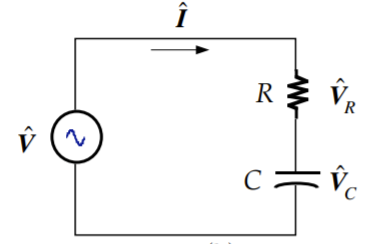
\includegraphics[scale = 0.8]{Images/RCSeries.PNG}
    \caption{RC series circuit.}
    \label{fig:RCSeries}
\end{figure}

We assume the source voltage phasor is purely real and equal to $\hat{V}_S$; equivalently, we will measure the phases of all oscillating quantities relative to the phase of the source voltage, which has phase zero. We first obtain the equivalent complex impedance of the RC series combination in our circuit: $$Z_{eq} = Z_R + Z_C = R + \frac{1}{j\omega C} = \frac{1+j\omega RC}{j\omega C}$$ 
Then the current phasor in the circuit is found using the definition of impedance: $$\hat{I} = \frac{\hat{V}}{Z_{eq}} = \frac{j\omega C}{1+j\omega RC}\hat{V}_S$$
The amplitude and phase of the current phasor are then given by \begin{equation*}
    \hat{I} = \frac{\omega C}{\sqrt{1+\omega^2R^2C^2}}V_S
\end{equation*}
and \begin{equation*}
    \phi = \text{arg}\hat{I} = \text{arg}(j\omega C) - \text{arg}(1+j\omega RC) + \text{arg}V_S = \frac{\pi}{2} - \tan^{-1}(\omega RC)
\end{equation*}
Now we can find the phasor voltage dropped across the resistor and capacitor by using the first form of the voltage divider equations: $$\hat{V}_R = \hat{I}R = \frac{j\omega RC}{1+j\omega RC}\hat{V}_S$$
and so $$|\hat{V}_R| = \frac{\omega RC}{\sqrt{1+\omega^2R^2C^2}}V_S$$
and $$\text{arg}\hat{V}_R = \text{arg}\hat{I}+\text{arg}R = \text{arg}\hat{I} = \frac{\pi}{2} - \tan^{-1}(\omega RC)$$
Similarly, for the capacitor, $$\hat{V}_C = \hat{I}Z_C = \frac{\hat{I}}{j\omega C} = \frac{1}{1+j\omega RC}\hat{V}_S$$ with amplitude $$|\hat{V}_C| = \frac{1}{\sqrt{1+\omega^2R^2C^2}}V_S$$
and phase $$\text{arg}\hat{V}_C = \text{arg}\hat{I} + \text{arg}Z_C = \text{arg}\hat{I} - \pi/2 = - \tan^{-1}(\omega RC)$$

\begin{figure}[H]
    \centering
    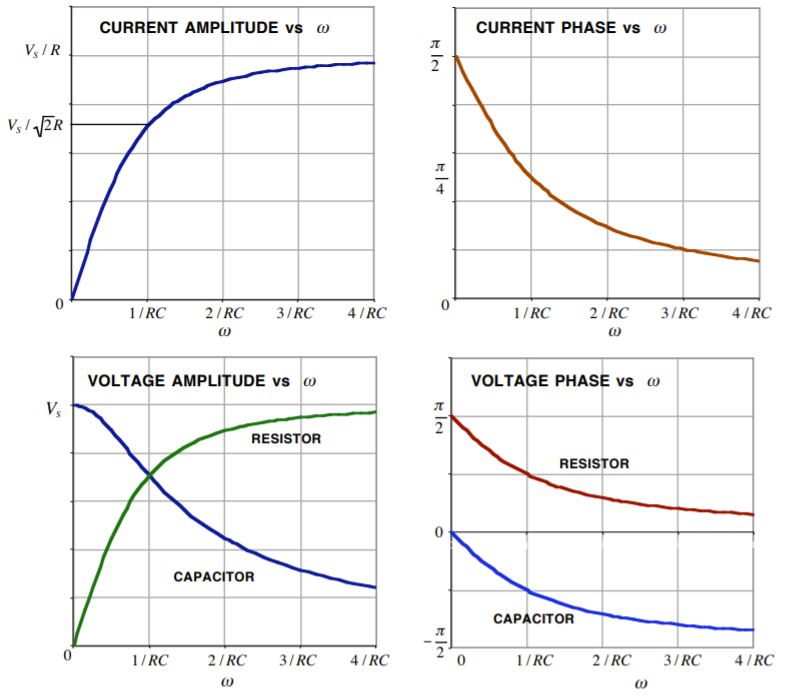
\includegraphics[scale = 0.8]{Images/RCGraph.PNG}
    \caption{Graphs of current and voltage amplitudes and phases as a function of angular frequency.}
    \label{fig:RCGraph}
\end{figure}

At low frequencies, $\omega \ll 1/RC$, the impedance $1/j\omega C$ of the capacitor is high, keeping the current amplitude small. The amplitude of the capacitor voltage is close to the source amplitude $V_S$ at these low frequencies. At high frequencies, $\omega \gg 1/RC$, the capacitor impedance is small and the amplitude of the current is limited by the resistor to an asymptotic value of $V_S/R$; the voltage drop across the resistor is approximately $V_S$, with the capacitor voltage drop being very small. At all frequencies the voltage signal dropped across the resistor always leads the voltage signal dropped across the capacitor by $\pi/2$ of phase. Since the phase difference is $\pi/2$, and we have the phasor relation $\hat{V}_S = \hat{V}_R + \hat{V}_C$, we have that $\hat{V}_R$ and $\hat{V}_C$ are orthogonal so pythagoras' theorem applies and $V_S^2 = V_C^2+V_R^2$.

\begin{rmk}[Analog filters]
    The RC circuit is useful as an \Emph{analog filter} to remove unwanted high or low frequency components from a time-continuous signal that contains a spectrum of frequencies. The filter can be said to have a \Emph{characteristic angular frequency} $\omega_C = 1/RC$ that can be seen as separating low frequencies from high frequencies. If we measure an output voltage signal across the resistor, we find that we strongly reject frequencies lying well below $\omega_C$ and retainthose that lie well above $\omega_C$. This is called a \Emph{high pass filter}. On the other hand, if we measure the output signal across the capacitor, we will have a \Emph{low pass filter} which also has its uses. Serious filter design usually requires cascading a number of RC or RLC circuits in a carefully designed series to get reasonable filter preformance. Such filters typically rely on inserting operational amplifiers in the cascade for successful implementation.
\end{rmk}

\begin{rmk}[Transient versus Steady State]
    The ideas of AC circuits that we have developed assume taht the AC source that drives the circuit has been connected for a time sufficiently long enough for exponentially decaying signals, called \Emph{transients}, to have died away, leaving only the simple \Emph{steady state} sinusoidal AC signals which have constant amplitude and phase, and which will persist unchanged until the source is disconnected at some future time, after which new transients emerge which bring down the steady state outputs smoothly and exponentially to zero. When we are thinking in terms of analog filters, we are thinking of the \Emph{steady state response} of the RC circuit.
\end{rmk}






%%%%%%%%%%%%%%%%%%%%%% Chapter 2.5
\chapter{The Series RLC Circuit}

\section{Differential Equation for the RLC circuit}

The RLC circuit is an AC circuit consisting of a capacitor resistor, and inductor all connected in series:

\begin{figure}[H]
    \centering
    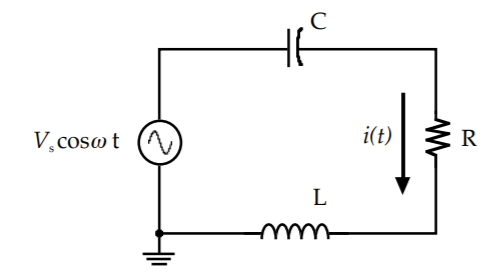
\includegraphics[scale = 0.8]{Images/RLCCircuit.PNG}
    \caption{The series RLC circuit, driven by an AC voltage source.}
    \label{fig:RLCCircuit}
\end{figure}

Applying Kirchhoff's loop rule (in the time domain) to the series RLC circuit in Figure \ref{fig:RLCCircuit} gives the following equation expressed in terms of the time-varying charge $q = \int idt$ stored in teh capacitor: \begin{equation*}
    L\frac{d^2q}{dt^2} + R\frac{dq}{dt} + \frac{q}{C} = V_s\cos\omega t
\end{equation*}
Note that this differential equation takes the form of a damped harmonic oscillator with a harmonic driving term: \begin{equation*}
    \ddot{x} + 2\gamma\dot{x} + \omega_0^2x = A\cos\omega t
\end{equation*}
The damping constant for us is $\frac{R}{2L}$, and the natural frequency of the undamped oscillator is $\omega_0 = \frac{1}{\sqrt{LC}}$. The RLC circuit also exhibits \Emph{resonance} (a large current amplitude when the driving frequency $\omega$ is equal to the natural frequency $\omega_0 = 1/\sqrt{LC}$).

\section{Resonance in the Series RLC Circuit}

We assume that the voltage source of Figure \ref{fig:RLCCircuit} has been connected for a long time so that any transient currents have died away, and the AC current in the circuit has reached its \Emph{steady state}. In terms of voltage and current phasors we can write our DE as \begin{equation*}
    \hat{I}(Z_C+Z_R+Z_L) = \hat{V}_s
\end{equation*}
where the impedance terms are $Z_C = 1/j\omega C, Z_R = R, Z_L = j\omega L$. Assigning a phase of zero to the source voltages, thus making $\hat{V}_s$ purely real, results in the following expression for the complex current amplitude in the circuit: \begin{equation*}
    \hat{I} = \frac{V_s}{\frac{1}{j\omega C}+R+j\omega L} = \frac{V_s}{R + j\left[\omega L - \frac{1}{\omega C}\right]}
\end{equation*}
The real amplitude $I$ and phase $\phi$ of the AC current are then \begin{equation*}
    I = \frac{V_s}{\sqrt{R^2 + \left[\omega L - \frac{1}{\omega C}\right]^2}};\;\;\phi = -\tan^{-1}\left[\frac{\omega L}{R} - \frac{1}{\omega RC}\right]
\end{equation*}
Note the current amplitude has a maximum, with respect to $\omega$, when $\omega = \omega_0 = \frac{1}{\sqrt{LC}}$. Thus, the natural angular frequency $\omega_0$ of the undamped oscillator is also the \Emph{resonance frequency} of the RLC circuit. At resonance, $\omega = \omega_0$, the current amplitude achieves its maximum value of $V_s/R$. Also the value of $\phi$ is zero at resonance; this means that the current is in phase with the source voltage when the current amplitude is maximum.

Since the current amplitude at resonance is proportional to $1/R$, changing $R$ while holding $L$ and $C$ fixed will change the height of the peak of the resonance curve without changing the resonance angular frequency, $\omega_0 = 1/\sqrt{LC}$.

One useful time scale in the RLC circuit is $1/\omega_0 = \sqrt{LC}$. Another comes from defining a dimensionless parameter $Q$ called the \Emph{quality factor} of the circuit: \begin{equation*}
    Q = \frac{\sqrt{L/C}}{R}
\end{equation*}
Circuits of given $L$ and $C$ with high $Q$ will have small values of $R$. Low-$Q$ circuits will have high values of $R$. We now define the \Emph{normalized angular frequency} $\overline{\omega}$: \begin{equation*}
    \overline{\omega} = \frac{\omega}{\omega_0} = \omega\sqrt{LC}
\end{equation*}
Using these definitions in the current amplitude and phase equations we can write \begin{equation*}
    I = \frac{V_s/R}{\sqrt{1+Q^2\left[\overline{\omega} - \frac{1}{\overline{\omega}}\right]^2}};\;\;\phi = -\tan^{-1}\left[Q\left(\overline{\omega} - \frac{1}{\overline{\omega}}\right)\right]
\end{equation*}

At resonance, the reactance of the RLC circuit disappears, and the circuit acts as a pure resistance (the impedance becomes purely real). The source voltage is dropped entirely across the resistor, and the current amplitude is $V_s/R$ irrespective of the values of $L$and $C$. It can be seen that increasing $Q$ for given values of $L$ and $C$, by decreasing the resistance $R$ in the circuit, will sharpen the resonance curve. 

\section{Voltage Characteristics}

We now wish to look at the AC voltage signals that appear across each of the elements in the RLC circuit, as represented by their three phasors: \begin{align*}
    \hat{V}_R &= \hat{I}Z_R = \hat{I}R \\
    \hat{V}_C &= \hat{I}Z_C = \hat{I}\frac{1}{j\omega C} \\
    \hat{V}_L &= \hat{I}Z_L = \hat{I}j\omega L
\end{align*}
The phasor $\hat{I} = I(\omega)e^{j\phi(\omega)}$ is common to all three expressions. It follows that \begin{itemize}
    \item The AC voltage signal dropped across the \Emph{resistor} has amplitude $V_R(\omega) = I(\omega)R$ and phase $\phi_R = \phi(\omega)$ (because $R$ is a positive real quantity)
    \item The AC voltage signal across the \Emph{capacitor} has amplitude $V_C(\omega) = I(\omega)/\omega C$ and phase $\phi_C = \phi(\omega) - \pi/2$ (because $\omega C$ is a positive real quantity and $1/j$ has phase $-\pi/2$)
    \item The AC voltage signal across the \Emph{inductor} has amplitude $V_L = \omega LI(\omega)$ and phase $\phi_L = \phi(\omega) + \pi/2$ (because $\omega L$ is a positive real quantity and $j$ has phase $\pi/2$)
\end{itemize}

Using the results for $I(\omega)$ and $\phi(\omega)$ found previously we then have \begin{align*}
    V_R(\omega) &= \frac{V_sR}{\sqrt{R^2+\left[\omega L-\frac{1}{\omega C}\right]^2}};\;\;\;\phi_R(\omega) = \phi(\omega) = -\tan^{-1}\left[\frac{\omega L}{R} - \frac{1}{\omega RC}\right] \\
    V_C(\omega) &= \frac{V_s/\omega C}{\sqrt{R^2+\left[\omega L-\frac{1}{\omega C}\right]^2}};\;\;\;\phi_C(\omega) = -\tan^{-1}\left[\frac{\omega L}{R} - \frac{1}{\omega RC}\right] - \frac{\pi}{2} \\
    V_L(\omega) &= \frac{\omega LV_s}{\sqrt{R^2+\left[\omega L-\frac{1}{\omega C}\right]^2}};\;\;\;\phi_L = -\tan^{-1}\left[\frac{\omega L}{R} - \frac{1}{\omega RC}\right] + \frac{\pi}{2}
\end{align*}





%%%%%%%%%%%%%%%%%%%%%% Chapter 2.6
\chapter{Impedances in Parallel}


%%%%%%%%%%%%%%%%%%%%%% Chapter 2.7
\chapter{Models of Real AC Sources; Th\'{e}venin's Theorem}


%%%%%%%%%%%%%%%%%%%%%% Chapter 2.8
\chapter{Power Dissipation}

